\documentclass[tikz,border=5mm,12pt]{standalone}
\usepackage[fontsize=16pt]{fontsize}
\usetikzlibrary{arrows.meta}
\usetikzlibrary{calc}

\newcommand\tokenfbox[1]{\fbox{\texttt{#1}\vphantom{\strut}}}
\def\arrowWidth{50mm}

\begin{document}
  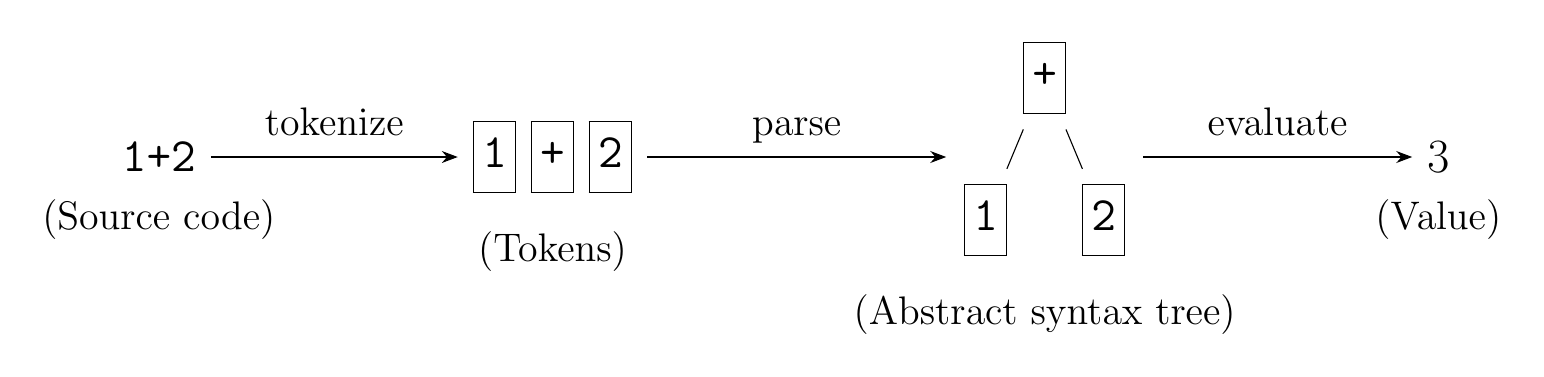
\begin{tikzpicture}[
    arrowtip/.style={
      -{Stealth[scale=1.2]}
    },
    level distance=18mm
  ]
    \def\plustoken{\tokenfbox{+}}
    \def\onetoken{\tokenfbox{1}}
    \def\twotoken{\tokenfbox{2}}

    \node (A) at (0*\arrowWidth,0) {\texttt{1+2}};
    \node (B) at (1*\arrowWidth,0) {\onetoken\ \plustoken\ \twotoken};
    \coordinate (C) at (2.25*\arrowWidth,0);
    \coordinate (CLeft) at (2*\arrowWidth,0);
    \coordinate (CRight) at (2.5*\arrowWidth,0);
    \coordinate[yshift=10mm] (CRoot) at (C);
    \coordinate[yshift=-10mm] (CChild) at (C);
    \node at (CRoot) {\plustoken}
      child {node {\onetoken}}
      child {node {\twotoken}};
    \node (D) at (3.25*\arrowWidth,0) {3};

    \draw[arrowtip] (A) -> node[above=-1mm] {\small tokenize\strut} (B);
    \draw[arrowtip] (B) -> node[above=-1mm] {\small parse\strut} (CLeft);
    \draw[arrowtip] (CRight) -> node[above=-1mm] {\small evaluate\strut} (D);

    \node[yshift=-8mm] at (A) {\small (Source code)};
    \node[yshift=-12mm] at (B) {\small (Tokens)};
    \node[yshift=-20mm] at (C) {\small (Abstract syntax tree)};
    \node[yshift=-8mm] at (D) {\small (Value)};
  \end{tikzpicture}
\end{document}
